% ===========================================================================
%  Policy sampling & MCTS planning on a Unified World Model (UWM)
%  ~10 minute talk.  Compiles standalone: figures are placeholder boxes you
%  replace with \includegraphics (see the \figbox macro / inline comments).
%
%  Build:  pdflatex policy-sampling-and-mcts.tex   (run twice for the outline)
% ===========================================================================
\documentclass[aspectratio=169]{beamer}
\usetheme{Madrid}
\usecolortheme{seahorse}
\setbeamertemplate{navigation symbols}{}
\setbeamertemplate{caption}[numbered]

\usepackage{amsmath,amssymb,bm}
\usepackage{graphicx}
\usepackage{xcolor}
\usepackage{tikz}
\usetikzlibrary{arrows.meta,positioning,calc}

\newcommand{\R}{\mathbb{R}}
\newcommand{\Exp}{\mathbb{E}}
\newcommand{\obs}{\bm{o}}
\newcommand{\act}{\bm{a}}
\newcommand{\state}{\bm{s}}
\newcommand{\zlat}{\bm{z}}
\newcommand{\prior}{\pi_{\mathrm{prior}}}

% ---- figure placeholder: a framed gray box with a caption ------------------
% Replace the whole \figbox{...} call with, e.g.:
%   \includegraphics[height=0.55\textheight]{figs/entropy_vs_ctxnoise.png}
\newcommand{\figbox}[2][0.55\textheight]{%
  \setlength{\fboxsep}{0pt}%
  \fcolorbox{gray!60}{gray!8}{%
    \begin{minipage}[c][#1][c]{0.86\textwidth}\centering
      \color{gray!70}\itshape [ figure placeholder ]\\[2pt]\small #2
    \end{minipage}}%
}

\title[Policy sampling \& MCTS on a UWM]{Policy sampling \& Monte-Carlo Tree Search\\on a Unified World Model}
\subtitle{Diverse rollouts as planning edges --- pushT}
\author{dreamerV4-UWM}
\date{\today}

\begin{document}

\begin{frame}[plain]\titlepage\end{frame}

\begin{frame}{Outline}
  \tableofcontents
\end{frame}

% ===========================================================================
\section{Context}
% ===========================================================================
\begin{frame}{Context: a Unified World Model as a generative prior}
  \textbf{Setup.} A single transformer denoiser models the \emph{joint}
  distribution of short clips of observations and actions in a frozen
  tokenizer's latent space (pushT; latents $\zlat\in\R^{256\times32}$,
  actions $\act\in\R^{2}$, context up to 64 frames).
  \vspace{0.4em}
  \begin{itemize}
    \item It is simultaneously a \textbf{policy} $p(\act\mid\obs)$, a
      \textbf{world model} $p(\obs'\mid\obs,\act)$, and a joint
      \textbf{imagination} model $p(\act,\obs'\mid\obs)$ --- all read off the
      same network by choosing \emph{which streams to denoise}.
    \item \textbf{Goal of this work.} Plan with \textbf{MCTS} where
      \emph{tree nodes are states} and \emph{tree edges are short rollouts}
      sampled from a prior policy $\prior$.
  \end{itemize}
  \vspace{0.4em}
  \begin{block}{The question that ties it together}
    A tree can only \emph{search} if its edges \emph{differ}.
    So: \emph{what makes $\prior$ diverse, and does that diversity reach the
    states the planner reasons about?}
  \end{block}
\end{frame}

% ===========================================================================
\section{Methods}
% ===========================================================================
\begin{frame}{Background: flow-matching denoiser \& noise levels}
  Each token stream carries a \textbf{cleanness} $\tau\in[0,1]$
  ($\tau=1$ clean, $\tau=0$ pure noise; noise level $n=1-\tau$). A noisy
  sample is the straight interpolation
  \[
    \bm{x}_\tau = \tau\,\bm{x} + (1-\tau)\,\bm\varepsilon,
    \qquad \bm\varepsilon\sim\mathcal N(0,I).
  \]
  The network returns a clean estimate $\hat{\bm x}$; the flow-matching
  \textbf{velocity} and an Euler step (step size $dt$) are
  \[
    \bm v(\bm x_\tau,\tau)=\frac{\hat{\bm x}-\bm x_\tau}{1-\tau},
    \qquad
    \bm x_{\tau+dt} = \bm x_\tau + \bm v\,dt .
  \]
  Sampling $=$ integrate $\tau:0\!\to\!1$ from a noise prior to a clean sample.
  Conditioning $=$ pin some frames/streams \emph{clean} ($\tau\approx1$) while
  integrating the rest.
\end{frame}

\begin{frame}{Three operating points on the noise square}
  \begin{columns}[T]
    \begin{column}{0.52\textwidth}
      Pick, \emph{per stream}, whether to integrate it or hold it. With clean
      observation context $\obs_{\le t}$:
      \begin{itemize}\small
        \item \textbf{Policy} $p(\act\mid\obs)$: horizon state held at noise
          ($n_{\state}\!=\!1$), action integrated $1\!\to\!0$.
        \item \textbf{Transition} $\obs' \!=\! f(\obs,\act)$: action given \&
          clean ($n_{\act}\!=\!0$), state integrated.
        \item \textbf{Imagine} $p(\act,\obs'\mid\obs)$: \emph{both} integrated
          $\;(1,1)\!\to\!(0,0)$ --- the \textbf{$\prior$ edge}.
      \end{itemize}
      \vspace{0.4em}
      One network, three samplers
      (\texttt{planning.rollout.\{policy,transition,imagine\}}).
    \end{column}
    \begin{column}{0.46\textwidth}
      \centering
      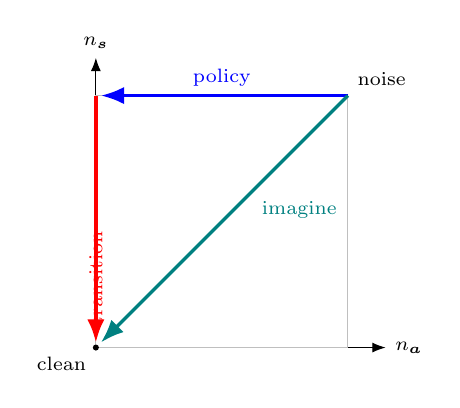
\begin{tikzpicture}[scale=3.2,>=Latex]
        \draw[->] (0,0)--(1.15,0) node[right]{\scriptsize $n_{\act}$};
        \draw[->] (0,0)--(0,1.15) node[above]{\scriptsize $n_{\state}$};
        \draw[gray!50] (0,0) rectangle (1,1);
        \node[below left] at (0,0) {\scriptsize clean};
        \node[above right] at (1,1) {\scriptsize noise};
        % policy: top edge n_state=1, n_act 1 -> 0
        \draw[->,blue,very thick] (1,1)--(0.02,1);
        \node[blue,above] at (0.5,1) {\scriptsize policy};
        % transition: left edge n_act=0, n_state 1 -> 0
        \draw[->,red,very thick] (0,1)--(0,0.02);
        \node[red,left,rotate=90] at (0,0.5) {\scriptsize transition};
        % imagine: diagonal
        \draw[->,teal,very thick] (1,1)--(0.02,0.02);
        \node[teal,below right] at (0.62,0.62) {\scriptsize imagine};
        \fill (0,0) circle (0.012);
      \end{tikzpicture}
      \\[-0.2em]{\scriptsize integration paths to the clean origin}
    \end{column}
  \end{columns}
\end{frame}

\begin{frame}{Diversity knobs (shared by all three samplers)}
  All stochasticity in a deterministic ODE comes from the \emph{prior draw} and
  the \emph{conditioning}. We expose:
  \begin{itemize}
    \item \textbf{Context-noise injection} $\rho\in[0,1]$ on the observation
      context, $\obs\leftarrow \tau_c\,\obs+(1-\tau_c)\bm\varepsilon$ with
      $\tau_c=1-\rho$.
      \emph{Honest}: tell the model $\sigma=\tau_c$ $\Rightarrow$ it returns the
      posterior under an uncertain state, $p(\act\mid\text{noisy }\obs)$.
      \emph{Mismatched}: corrupt but announce clean (out-of-distribution).
    \item \textbf{Action temperature} $T$: scale the action prior,
      $\act_0\sim\mathcal N(0,T^2 I)$ (transports a wider prior; $T\!\neq\!1$ is
      mildly off-distribution).
    \item \textbf{Steps} $K$: number of Euler steps (fidelity vs.\ cost).
  \end{itemize}
  \begin{block}{Diversity metrics}
    Action spread via Gaussian differential entropy
    $H=\tfrac12\log\!\big((2\pi e)^d|\Sigma|\big)$ and per-dim std;
    \textbf{downstream state spread} via the per-sample std of imagined latents.
  \end{block}
\end{frame}

\begin{frame}{Implementation notes}
  \begin{itemize}
    \item \textbf{Everything in \texttt{bf16} autocast.} fp32 forwards OOM at
      planning batch sizes and are ${\sim}3.5\times$ slower; bf16 world-model
      reconstruction matches fp32 (latent MSE $0.0043$ vs.\ $0.0047$).
    \item \textbf{Latent-space planning.} The whole search runs on tokenizer
      latents; decode only for visualization.
    \item \textbf{Batched candidate pools.} A node draws all its candidate
      edges in \emph{one} batched \texttt{imagine} call (amortizes the
      transformer forward over the pool).
    \item \textbf{Pluggable} edge sampler and reward
      (\texttt{planning.\{rollout,reward,mcts\}}); reward is a basic
      goal-distance for now (no learned critic yet).
  \end{itemize}
\end{frame}

% ===========================================================================
\section{Policy: diversity for planning}
% ===========================================================================
\begin{frame}{Policy mode: experiment design}
  \textbf{Policy marginal} $p(\act_t\mid\obs_{\le t})$: clean context, horizon
  state held at noise, action integrated. We ask whether the user's first idea
  --- \emph{inject noise into the context} --- yields more diverse (higher
  entropy) trajectories, and whether that diversity \emph{reaches the states}.
  \vspace{0.6em}
  \begin{itemize}
    \item Sweep context noise $\rho$ (honest vs.\ mismatched) and temperature $T$.
    \item Measure (i) action entropy/std, (ii) \textbf{downstream latent-state
      spread} of imagined rollouts, (iii) mode structure of the 2-D action cloud.
  \end{itemize}
\end{frame}

\begin{frame}{Result 1 --- context noise raises action diversity}
  \begin{columns}[T]
    \begin{column}{0.5\textwidth}
      \figbox[0.5\textheight]{action clouds + entropy vs.\ $\rho$ (honest vs.\ mismatched)}
      % \includegraphics[height=0.5\textheight]{figs/entropy_vs_ctxnoise.png}
    \end{column}
    \begin{column}{0.5\textwidth}
      \textbf{Honest context noise widens $p(\act\mid\obs)$ monotonically.}
      \begin{center}\small
      \begin{tabular}{ccc}
        \hline
        $\rho$ & $H$ (honest) & $H$ (mismatch)\\\hline
        0.00 & $-11.66$ & $-11.66$\\
        0.30 & $-9.97$  & $-9.93$\\
        0.50 & $-8.86$  & $-8.71$\\\hline
      \end{tabular}
      \end{center}
      \begin{itemize}\small
        \item Honest noise is the \emph{principled} knob: it asks the model for
          its posterior under an uncertain state.
        \item Temperature $T$ also raises $H$ ($-11.8\!\to\!-11.3$ for
          $T\!:\!0.5\!\to\!2$) but is mildly OOD.
      \end{itemize}
    \end{column}
  \end{columns}
\end{frame}

\begin{frame}{Result 2 --- but does diversity reach the \emph{states}?}
  \begin{columns}[T]
    \begin{column}{0.5\textwidth}
      \figbox[0.5\textheight]{normalized action spread vs.\ latent-state spread vs.\ $\rho$}
      % \includegraphics[height=0.5\textheight]{figs/state_coverage.png}
    \end{column}
    \begin{column}{0.5\textwidth}
      \textbf{The key planning metric is state coverage, not action entropy.}
      \begin{center}\small
      \begin{tabular}{ccc}
        \hline
        $\rho$ & action $|\mathrm{std}|$ & latent spread\\\hline
        0.00 & 0.0026 & 0.026\\
        0.50 & 0.0066 & 0.031\\
        0.70 & 0.0424 & 0.058\\\hline
      \end{tabular}
      \end{center}
      \begin{itemize}\small
        \item At low noise the policy is \textbf{near-deterministic} and the
          world model \emph{contracts} diverse actions onto one trajectory.
        \item Only with enough honest noise do the \emph{states} branch.
      \end{itemize}
    \end{column}
  \end{columns}
\end{frame}

\begin{frame}{Policy: conclusions}
  \begin{itemize}
    \item \textbf{Yes}, injecting (honest) context noise produces more diverse,
      higher-entropy trajectories.
    \item \textbf{But action entropy is not the target.} Diverse actions that
      lead to the same state give a planner nothing to choose between.
    \item The binding quantity is \textbf{controllable state diversity}; on this
      checkpoint it is small at low noise --- a direct constraint on what MCTS
      can search over.
  \end{itemize}
  \vspace{0.4em}
  \begin{block}{Takeaway feeding into the planner}
    The diversity knobs become \emph{planner hyper-parameters}: they set how
    much the tree is allowed to branch.
  \end{block}
\end{frame}

% ===========================================================================
\section{MCTS planning}
% ===========================================================================
\begin{frame}{MCTS: states, edges, returns}
  \textbf{Continuous-action, generative MCTS.}
  \begin{itemize}
    \item \textbf{Node} $=$ state $\state$: a latent observation/action history
      the denoiser conditions on (the context window).
    \item \textbf{Edge} $=$ a short rollout $\xi=(\act_{0:H},\zlat_{0:H})\sim
      \prior(\cdot\mid\state)$ (one \texttt{imagine} call). Applying it advances
      the window to a child node $\state'$.
    \item \textbf{Reward} $r(\zlat)$: basic negative latent distance to a goal
      frame, $r(\zlat)=-\lVert\zlat-\zlat_{\mathrm{goal}}\rVert^2/\kappa$.
    \item \textbf{Edge return} (per-frame discount $\gamma$):
      \[ g(\xi)=\sum_{h=0}^{H-1}\gamma^{h}\,r(\zlat_h). \]
  \end{itemize}
  Because actions are continuous and edges are \emph{sampled} (not enumerable),
  the tree needs \emph{progressive widening}.
\end{frame}

\begin{frame}{MCTS: the algorithm I implemented}
  Each simulation descends root$\to$leaf, expands one node, and backs up:
  \begin{enumerate}\small
    \item \textbf{Progressive widening.} A node visited $N(\state)$ times is
      allowed $\big\lceil C\,N(\state)^{\alpha}\big\rceil$ children. If under
      budget, \emph{reveal} the next edge from a fixed candidate \textbf{pool}
      (drawn once, batched, on first visit) and stop to evaluate it.
    \item \textbf{Selection.} Otherwise pick the child maximizing a UCB score
      \[
        e^\star=\arg\max_{e}\;\;
        \underbrace{\widetilde{Q}(e)}_{\text{min--max norm.}}
        \;+\;c\,\frac{\sqrt{N(\state)}}{1+N(e)},\qquad
        \widetilde Q=\frac{Q-Q_{\min}}{Q_{\max}-Q_{\min}},
      \]
      with $Q(e)=W(e)/N(e)$; descend to its child.
    \item \textbf{Leaf value.} New leaf valued by $V_{\text{leaf}}$
      ($0$, or a few short imagined simulation rollouts for a bootstrap).
    \item \textbf{Backup} along the path, edge length $H$:
      \[ G \leftarrow g(e)+\gamma^{H}\,G,\qquad
         N(e)\!\mathrel{+}=\!1,\;\; W(e)\!\mathrel{+}=\!G. \]
  \end{enumerate}
  \textbf{Recommendation:} the \emph{most-visited} root edge $\to$ action chunk.
\end{frame}

\begin{frame}{MCTS: why these choices}
  \begin{itemize}
    \item \textbf{Progressive widening} is the standard answer to an infinite
      (continuous / sampled) action set: grow children with visits instead of
      enumerating.
    \item \textbf{Candidate pool} batches all of a node's edge samples into one
      forward --- the dominant cost is the transformer, not the tree.
    \item \textbf{Min--max $Q$ normalization} (MuZero-style): rewards live on an
      arbitrary negative-distance scale, so $Q$ must be normalized for $c$ to
      behave.
    \item \textbf{Diversity knobs forwarded to the edge sampler}
      ($\rho$, $T$): this is exactly where the policy study feeds the planner.
    \item Edge sampler and reward are \textbf{pluggable} (joint \texttt{imagine}
      by default; a two-stage policy$\to$transition $\prior$ is a drop-in).
  \end{itemize}
\end{frame}

\begin{frame}{MCTS: results}
  \begin{columns}[T]
    \begin{column}{0.5\textwidth}
      \figbox[0.5\textheight]{decoded planned rollout (start ctx $\to$ rollout $\to$ goal)}
      % \includegraphics[height=0.5\textheight]{figs/mcts_rollout.png}
    \end{column}
    \begin{column}{0.5\textwidth}
      \textbf{Goal-reaching, reachable goal, diversity injected
      ($\rho{=}0.5,\,T{=}1.5$).}
      \begin{itemize}\small
        \item Planned terminal reward $\mathbf{-2.45}$ vs.\ random
          $-2.79\pm0.38$ $\;\Rightarrow\;$ \textbf{gain $+0.34$} (${\sim}0.9\sigma$).
        \item Budget: 48 simulations, 31 batched forwards, ${\sim}59$\,s.
        \item \textbf{Search correctness} (controllable mock world, known
          optimum): visits concentrate on the max-reward branch; planned
          terminal $=6.0/6.0$.
      \end{itemize}
      \vspace{0.3em}
      \figbox[0.18\textheight]{root edge visit counts vs.\ $Q$}
      % \includegraphics[height=0.18\textheight]{figs/visits_vs_Q.png}
    \end{column}
  \end{columns}
\end{frame}

\begin{frame}{MCTS: conclusions}
  \begin{itemize}
    \item The planner is \textbf{correct} (verified in isolation) and gives a
      real gain over random \emph{when} (a) edges are diverse and (b) the goal
      is reachable within the planning horizon.
    \item With a far / unreachable goal or near-deterministic edges, the gain
      washes out --- the limit is \textbf{model controllability}, not the search.
    \item Cost is dominated by un-cached transformer forwards on the context.
  \end{itemize}
  \vspace{0.4em}
  \begin{block}{Next steps}
    \begin{enumerate}\small
      \item \textbf{KV-cached edges} (build on the hybrid chunk sampler) ---
        deeper trees, real-time receding-horizon control.
      \item \textbf{Controllability probe}: quantify $\partial\state/\partial\act$
        over the horizon to plan only at high-leverage states.
      \item \textbf{Learned reward / critic} to replace the basic goal distance.
    \end{enumerate}
  \end{block}
\end{frame}

% ===========================================================================
\begin{frame}{Summary}
  \begin{itemize}
    \item One UWM gives policy, world model, and joint imagination by choosing
      which streams to denoise.
    \item \textbf{Honest context noise} makes the policy diverse; the diversity
      that matters is \textbf{state coverage}, which the world model can
      contract.
    \item A \textbf{continuous-action, progressive-widening MCTS} plans over
      latent states with $\prior$ rollouts as edges; it is correct and helps
      when the model affords controllable, reachable branching.
  \end{itemize}
  \vspace{0.8em}
  \centering\large Thank you --- questions?
\end{frame}

\end{document}
